\documentclass[tikz, border=10pt]{standalone}
\usepackage{tikz}
\usepackage{amsmath}
\usetikzlibrary{automata, positioning, arrows.meta}

\begin{document}
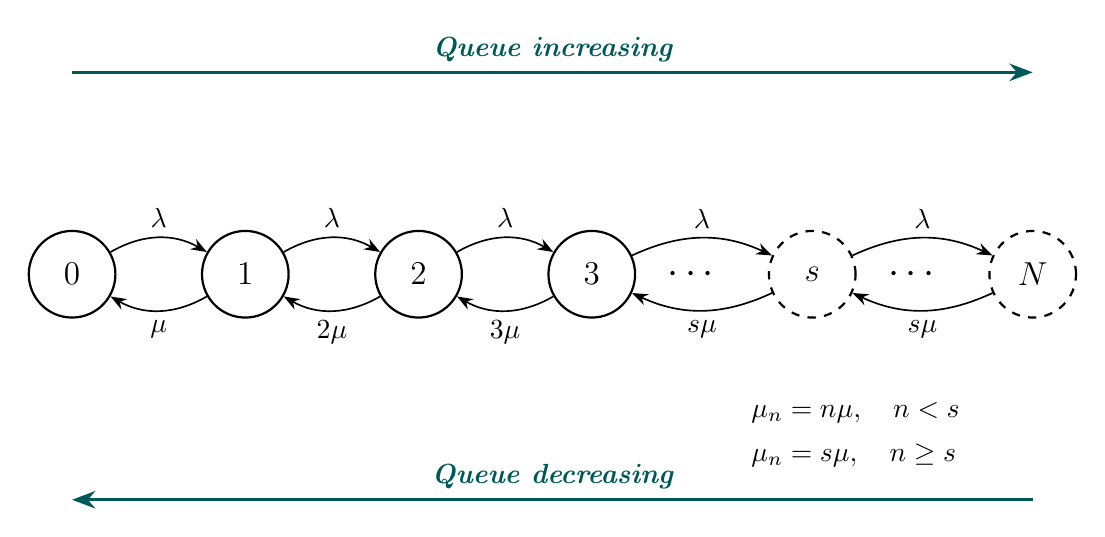
\begin{tikzpicture}[
        node distance=2.2cm,
        every state/.style={circle, draw, thick, minimum size=1.1cm, font=\large\bfseries},
        >=Stealth, auto, semithick
    ]

    %% ---- Solid states: 0, 1, 2, 3 ----
    \node[state] (0) {$0$};
    \node[state, right of=0] (1) {$1$};
    \node[state, right of=1] (2) {$2$};
    \node[state, right of=2] (3) {$3$};

    %% ---- Dashed states: s, N ----
    \node[state, dashed, right of=3, node distance=2.8cm] (s) {$s$};
    \node[state, dashed, right of=s, node distance=2.8cm] (N) {$N$};

    %% ---- Dots ----
    \node[right of=3, node distance=1.3cm, font=\Large] {$\cdots$};
    \node[right of=s, node distance=1.3cm, font=\Large] {$\cdots$};

    %% ---- Forward transitions (lambda) ----
    \draw[->] (0) to[bend left=30] node[above] {$\lambda$} (1);
    \draw[->] (1) to[bend left=30] node[above] {$\lambda$} (2);
    \draw[->] (2) to[bend left=30] node[above] {$\lambda$} (3);
    \draw[->] (3) to[bend left=25] node[above] {$\lambda$} (s);
    \draw[->] (s) to[bend left=25] node[above] {$\lambda$} (N);

    %% ---- Backward transitions (variable mu) ----
    \draw[->] (1) to[bend left=30] node[below] {$\mu$}   (0);
    \draw[->] (2) to[bend left=30] node[below] {$2\mu$}  (1);
    \draw[->] (3) to[bend left=30] node[below] {$3\mu$}  (2);
    \draw[->] (s) to[bend left=25] node[below] {$s\mu$}  (3);
    \draw[->] (N) to[bend left=25] node[below] {$s\mu$}  (s);

    %% ---- Directional arrows ----
    \draw[->, thick, color=teal!70!black, line width=1.2pt]
    ([yshift=2.0cm] 0.north) -- ([yshift=2.0cm] N.north)
    node[midway, above, font=\itshape\bfseries, color=teal!70!black] {Queue increasing};

    \draw[->, thick, color=teal!70!black, line width=1.2pt]
    ([yshift=-2.3cm] N.south) -- ([yshift=-2.3cm] 0.south)
    node[midway, above, font=\itshape\bfseries, color=teal!70!black] {Queue decreasing};

    %% ---- Piecewise formula (above the decreasing arrow) ----
    \node[align=left, anchor=north west, font=\normalsize]
    at ([xshift=1.5cm, yshift=-1.1cm] 3.south east) {
        $\mu_n = n\mu, \quad n < s$ \\[4pt]
        $\mu_n = s\mu, \quad n \geq s$
    };

\end{tikzpicture}
\end{document}